\documentclass[11pt]{article}
\author{Tianyu Du}
\title{MAT223 Linear Algebra Tophat Chapter 4}
\date{\today}
\usepackage{amsmath}
\usepackage{amssymb}
\usepackage{amsthm}
\usepackage{enumerate}

\usepackage{fancyhdr}
\pagestyle{fancy}
\lhead{Tianyu Du}
\rhead{\today}
\usepackage[
	type={CC},
	modifier={by-nc-sa},
	version={3.0},
]
{doclicense}

\newtheorem{theorem}{Theorem}
\newtheorem{definition}{Definition}
\newtheorem{proposition}{Proposition}

\newcommand{\norm}[1]{\lVert #1 \rVert}
\newcommand{\proj}[2]{proj_{\vec{#2}} \vec{#1}}
\newcommand{\re}[1]{\mathbb{R}^#1}
\newcommand{\ma}[2]{\mathbb{M}_{#1 \times #2}}

\begin{document}
	\maketitle
	\doclicenseThis
	\section{The Rank Theorems}
	\subsection{Subspaces of $\mathbb{R}^n$}
	\begin{theorem}[Subspace Theorem]
		Let $S$ be a subspace of $\mathbb{R} ^ n$. If $S$ is spanned by $m$ vectors, and contains $k$ linearly independent vectors, then $k \leq m$.
	\end{theorem}
	\subsection{Bases}
	\begin{theorem}
		Let $S \neq \{\vec{0}\}$ be a subspace pf $\mathbb{R} ^ n$. Then there's a basis for S.
	\end{theorem}
	\begin{theorem}
		A basis for a subspace $S \subseteq \mathbb{R}^n$ can only have one size.
	\end{theorem}
	\begin{definition}[Dimension]
		The \textbf{dimension} $dim S$ of a nonzero subspace $v$ is $\sharp B$ for any basis B of S.
	\end{definition}
	\subsection{Expansions and Orthogonalization}
	\begin{theorem}[Gram-Schmidt Orthonormalization Procedure]
		Let ${\vec{b}_1,\dots,\vec{b}_k} \subseteq \re{n}$ be a basis for a subspace $S$. Define
		\begin{align*}
			\vec{w_1} = \hat{b_1} \\
			\vec{w_2} = \hat{x_2}, \vec{x_2} = \vec{b_2} - \proj{b_2}{w_1} \\
			\vec{w_k} = \hat{x_k}, \vec{x_k} = \vec{b_k} - \sum_{i=1}^{k-1}\proj{b_k}{w_i}
		\end{align*}
		The vectors $\{\vec{w_i}\}_1^k$ produced as above are an \textbf{orthonormal basis} for $S$.
	\end{theorem}
	\subsection{Rank Unification}
	\begin{definition}[Rank]
		The \textbf{rank} of a matrix A, denoted $rank(A)$ is the number of pivots in A.
	\end{definition}
	\begin{theorem}[Rank Theorem]
		Let A be an $m\times n$ matrix with rank r. Then
		\[
			dim(col(A)) = dim(row(A)) = r
		\]
		Moreover, if A ~ R where R is in row-echelon form then
		\begin{enumerate}
			\item The r nonzero rows of R form a basis for row(A).
			\item The r pivot columns of A form a basis for col(A).
		\end{enumerate}
	\end{theorem}
	\begin{theorem}[Rank-Nullity Theorem]
		Let A be a $m \times n$ matrix. Then
		\[
			rank(A) + dim(ker(A)) = n
		\]
		We call $dim(ker(A))$ as \textbf{nullity} of A.
	\end{theorem}
	\paragraph{Note} The \emph{rank-nullity theorem} is a way to quantitatively characterize how far a given matrix might be from having $A\vec{x} = \vec{b}$ be uniquely solvable.
	\paragraph{Note} To find a basis for kernel space, we write all basic variables of system $A\vec{x} = \vec{0}$ in terms of free variables.
	\begin{theorem}[Rank Inequalities]
		Let A be a $m \times n$ matrix, we have
		\[
			rank(A) \leq min(m,n)
		\]
	\end{theorem}
	\begin{definition}[Maximal Rank]
		A $m \times n$ matrix has \textbf{full rank} or \textbf{maximal rank} when $rank(A) = min(m,n)$
	\end{definition}
	\paragraph{Note} A square matrix with full rank must be invertible.
	\begin{theorem}
		Let A, B and C be matrices such that the products below are well-defined. Then
		\begin{enumerate}
			\item $col(AB) \subseteq col(A)$
			\item $row(CA) \subseteq row(A)$
		\end{enumerate}
		In the above $\subseteq$ will simply be $=$ when B or C respectively is invertible.
	\end{theorem}
	\begin{theorem}
		If A and B are two matrices whose product is defined then
		\[
			rank(AB) \leq min(rank(A), rank(B))
		\]
	\end{theorem}
	\subsection{Maximal Rank}
	\paragraph{Note} If A were square, then A having full rank ensures that system $A\vec{x} = \vec{b}$ is always \emph{uniquely solvable}.
	\begin{theorem}[Rank = $\sharp$ of Columns]
		Let A be a $m \times n$ matrix, the following statements are equivalent.
		\begin{enumerate}
			\item $rank(A) = n$.
			\item $row(A) = \re{n}$.
			\item Columns of A are linearly independent.
			\item $A^{T}$ A is invertible.
			\item $\exists C \in \ma{n}{m}$ such that $C*A = I_n$.
			\item $A\vec{x} = \vec{0}$ has only trivial solution.
		\end{enumerate}
	\end{theorem}
	\begin{theorem}[Rank = $\sharp$ of rows]
		Let A be $m \times n$. The following are equivalent statements.
		\begin{enumerate}
			\item $rank(A) = m$.
			\item $col(A) = \re{m}$.
			\item Rows of A are linearly independent.
			\item $A A^{T}$ is invertible.
			\item $\exists D \in \ma{n}{m}$ such that $A*D = I_m$.
			\item $A\vec{x} = \vec{b}$ holds for all $\vec{b} \in \re{m}$.
		\end{enumerate}
	\end{theorem}
	\section{The Fundamental Theorem of Linear Algebra}
	\subsection{Prelude: Orthogonal Complements}
	\begin{definition}
		Let $S \subseteq \re{n}$ be a subspace, define $S^\perp \in \re{n}$ as
		\[
		S^\perp = \{\vec{u} \in \re{n} \vert \vec{u} \cdot \vec{v} = 0, \forall \vec{v} \in S\}
		\] $S^\perp$ is the the \textbf{orthogonal complement} of $S$ in $\re{n}$.
	\end{definition}
	\begin{theorem}
		Let $\vec{v} \in \re{n}$, and let $S \subseteq \re{n}$ be a subspace. \newline Then there are vectors
		\begin{align*}
			\vec{s} \in S \\
			\vec{s_{\perp}} \in S^\perp \\
		\end{align*}
		such that,
		\[
			\vec{v} = \vec{s} + \vec{s_{\perp}}
		\]
	\end{theorem}
	\paragraph{Explanation} \underbar{Vectors can be expressed in terms of pieces in orthogonal space.}
	\paragraph{Note} This fact is expressed as $\re{n} = S \bigoplus S^\perp$ (\emph{direct sum}).
	\begin{proof}
		Since $S \in \re{n}$ is a subspace, and every subspace has basis. \\
		Let $B_1$ be a basis of $S$. \\
		Let $B = \{\vec{s_i}\}_1^{dimS}$ be the orthonormal basis of S generated from $B_1$ via GSO. \\
		
		So that, $\vec{s_i} \cdot \vec{s_j} = \begin{cases}
 			1, i = j \in \mathbb{Z}_1^{dimS} \\
 			0, i \neq j \in \mathbb{Z}_1^{dimS} \\ 
 			\end{cases}$ \\
 			
 		For a vector $\vec{v} \in \re{n}$ \\
 	
 		Let $\vec{s} = \sum_{i=1}^{dimS} (\vec{v} \cdot \vec{s_i})\vec{s_i}$. $\vec{s}$ is a linear combination of vectors in the orthonormal basis $B$ of space S, so obviously, $\vec{s} \in S$.\\
 	
		Define $\vec{s_{\perp}} = \vec{v} - \vec{s}$.\\
		
		$\forall j \in \mathbb{Z}_1^{dimS}$, Consider $\vec{s_\perp} \cdot \vec{s_j}.$ \\
		
		$\vec{s_\perp} \cdot \vec{s_j} = (\vec{v} - \vec{s}) \cdot \vec{s_j} = \vec{v} \cdot \vec{s_j} - \sum_{i=1}^{dimS}(\vec{v} \cdot \vec{s_i} \cdot \vec{s_i} \cdot \vec{s_j}) = \vec{v} \cdot \vec{s_j} - \vec{v} \cdot \vec{s_j} = 0$ \\
		
		So that, $\vec{s_\perp} \in S^\perp$.
		
		By definition of $\vec{s_\perp}$ above, $\vec{v} = \vec{s} + \vec{s_\perp} \in \re{n}$, where $\vec{s} \in S \land \vec{s_\perp} \in S^\perp$. 
	\end{proof}
	\subsection{The Fundamental Theorem of Linear Algebra}
	\begin{proposition}
		Let $A \in \ma{m}{n}(\mathbb{R})$. Then,
		\[
			Col(A^T)^\perp = Ker(A)
		\]
	\end{proposition}
	\begin{proof}
		\textbf{Part1}\\
		
		Let $\vec{v} \in Ker(A)$, we have $A\vec{v} = \vec{0}$ \\
		
		So that, $\begin{bmatrix}
				Row_1(A) \vec{v} \\
				Row_2(A) \vec{v} \\
				\vdots \\
				Row_m(A) \vec{v} \\
			\end{bmatrix} = \vec{0}$ \\
		
		So that, $\vec{v}$ is orthogonal to all rows of A. \\
		
		So that, $\vec{v} \in Row(A)^\perp \land Row(A) = Col(A^T)$ \\
		
		$\vec{v} \in Col(A^T)^\perp$\\
		
		We have, $\vec{v} \in Ker(A) \implies \vec{v} \in Col(A^T)^\perp$ \\
		
		So that, $Ker(A) \subseteq Col(A^T)^\perp$ \\
		
		\textbf{Part2}\\
		
		Let $\vec{v} \in Col(A^T)^\perp$ \\
		
		Since $Col(A^T) = Row(A)$, we have $\vec{v} \in Row(A)^\perp$ \\
		
		So that, $Row_j(A) \cdot \vec{v} = 0, \forall j \in \mathbb{Z}_1^m$ \\
		
		So that, $A\vec{v} = \vec{0}$, which implies $\vec{v} \in Ker(A)$. \\
		
		We have, $\vec{v} \in Col(A^T)^\perp \implies \vec{v} \in Ker(A) $ \\
		
		Equivalently, $Col(A^T)^\perp \subseteq Ker(A)$ \\
		
		Now we have $Ker(A) \subseteq Col(A^T)^\perp \land Col(A^T)^\perp \subseteq Ker(A) \iff Ker(A) = Col(A^T)^\perp \iff Ker(A)^\perp = Col(A^T)$\\
	\end{proof}
	
	\begin{theorem}[The Fundamental Theorem of Linear Algebra]
		Let $A \in \ma{m}{n}(\mathbb{R})$ \\
		Then, (i) $Col(A^T) = Ker(A)^\perp$ \\
		
		(ii) $\re{n} = Col(A^T) \bigoplus Ker(A)$ \\
		
		And, $\forall \vec{v} \in Col(A)$, we have, $A\vec{x} = \vec{b}$ solved by $\vec{x} = \vec{p} + \vec{v_h}$, where $\vec{p} \in Row(A)$ and $\vec{v_h} \in Ker(A)$.\\
		 
	\end{theorem}
	\paragraph{Explanation} (ii): \textbf{Orthogonal decomposition} of $\re{n}$ into the \emph{null space} and the \emph{row space} of matrix A.
	\paragraph{Note} For the counter part of this theorem over $\re{m}$, consider matrix $B = A^T$ and proof via the same vein.
	
	\subsection{The Diagrams}
	\paragraph{} Let matrix $A \in \ma{m}{n}(\mathbb{R})$.
	\subsubsection{Decomposition of $\re{n}$}
	\paragraph{Representation} $\re{n} = Row(A) \bigoplus Ker(A)$.
	\begin{figure*}[h]
		\centering
		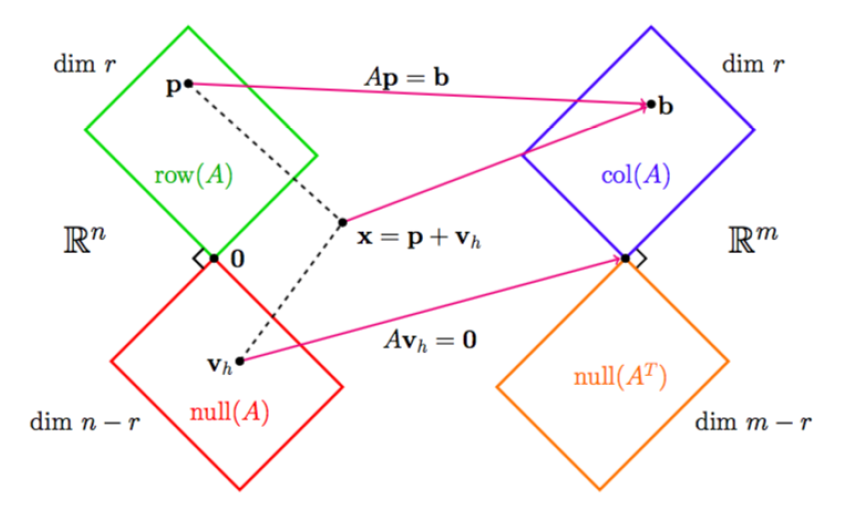
\includegraphics[width=\linewidth]{223_pic/decomposition_rn}
		\caption{The decomposition of $\re{n}$}
	\end{figure*}
	
	\subsubsection{Decomposition of $\re{m}$}
	\paragraph{Representation} $\re{m} = Col(A) \bigoplus Ker(A^T)$.
	\begin{figure*}[h]
		\centering
		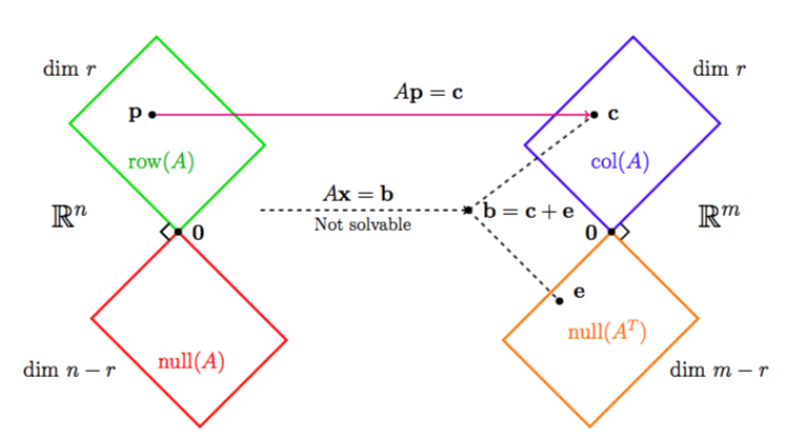
\includegraphics[width = \linewidth]{223_pic/decomposition_rm}
		\caption{The decomposition of $\re{m}$}
	\end{figure*}
\end{document}




































